\documentclass[11pt,a4paper]{article}
\usepackage[utf8]{inputenc}
\usepackage[french]{babel}
\usepackage{graphicx}
\usepackage{geometry}
\usepackage{hyperref}
\usepackage{listings}
\usepackage{xcolor}
\usepackage{fancyhdr}
\usepackage{float}
\usepackage{booktabs}

\geometry{margin=2cm, top=1.5cm, bottom=1.5cm}
\pagestyle{fancy}
\fancyhf{}
\fancyhead[L]{\small Pipeline Data Engineering}
\fancyhead[R]{\small \thepage}
\renewcommand{\headrulewidth}{0.4pt}

\hypersetup{colorlinks=true, linkcolor=blue, urlcolor=cyan}
\definecolor{codebg}{rgb}{0.95,0.95,0.95}
\lstset{basicstyle=\ttfamily\small, breaklines=true, backgroundcolor=\color{codebg}}

\title{\Large \textbf{Pipeline Data Engineering\\Collecte et Visualisation de Cryptomonnaies}}
\author{\large Asma Sebai}
\date{\large Avril 2026}

\begin{document}

\maketitle

{\small \tableofcontents}
\newpage

% ===== 1. CONTEXTE =====
\section{Contexte et Objectif}

Le marché des cryptomonnaies, caractérisé par une volatilité élevée 24h/24, nécessite des outils d'analyse robustes. Ce projet démontre la maîtrise complète d'un \textbf{pipeline Data Engineering production-ready} intégrant Apache Spark.

\textbf{Objectifs :}
\begin{itemize}[noitemsep]
    \item Collecter automatiquement les prix de 5 cryptomonnaies majeures
    \item Traiter les données avec un moteur dual-engine Pandas/Spark
    \item Orchestrer le pipeline automatiquement
    \item Visualiser les résultats via un dashboard professionnel (accessible en ligne)
\end{itemize}

\textbf{Technologies clés :} Python, PostgreSQL, Apache Spark, Kafka, Streamlit, Docker, Cloud (Neon, Streamlit Cloud)

% ===== 2. SOURCES DE DONNÉES =====
\section{Sources de Données}

\textbf{Source 1 -- CoinGecko API (Batch) :} API REST publique, 5 cryptomonnaies, appels toutes les 10 minutes, format JSON. Données : prix, market cap, volumes, variations 24h.

\textbf{Source 2 -- Apache Kafka (Streaming) :} Topic \texttt{crypto\_prices}, messages toutes les 5 secondes, format JSON. Simule un flux temps réel de prix avec variations aléatoires (±2\%).

\textbf{Volume :} $\sim$5 000 lignes batch + $\sim$600 000 lignes streaming potentielles sur 7 jours = \textbf{$\sim$605 000 enregistrements totaux}.

% ===== 3. ARCHITECTURE =====
\section{Architecture du Pipeline}

Le pipeline suit une architecture ETL enrichie d'une couche streaming, dual-engine Pandas/PySpark et orchestration automatisée.

\begin{figure}[H]
    \centering
    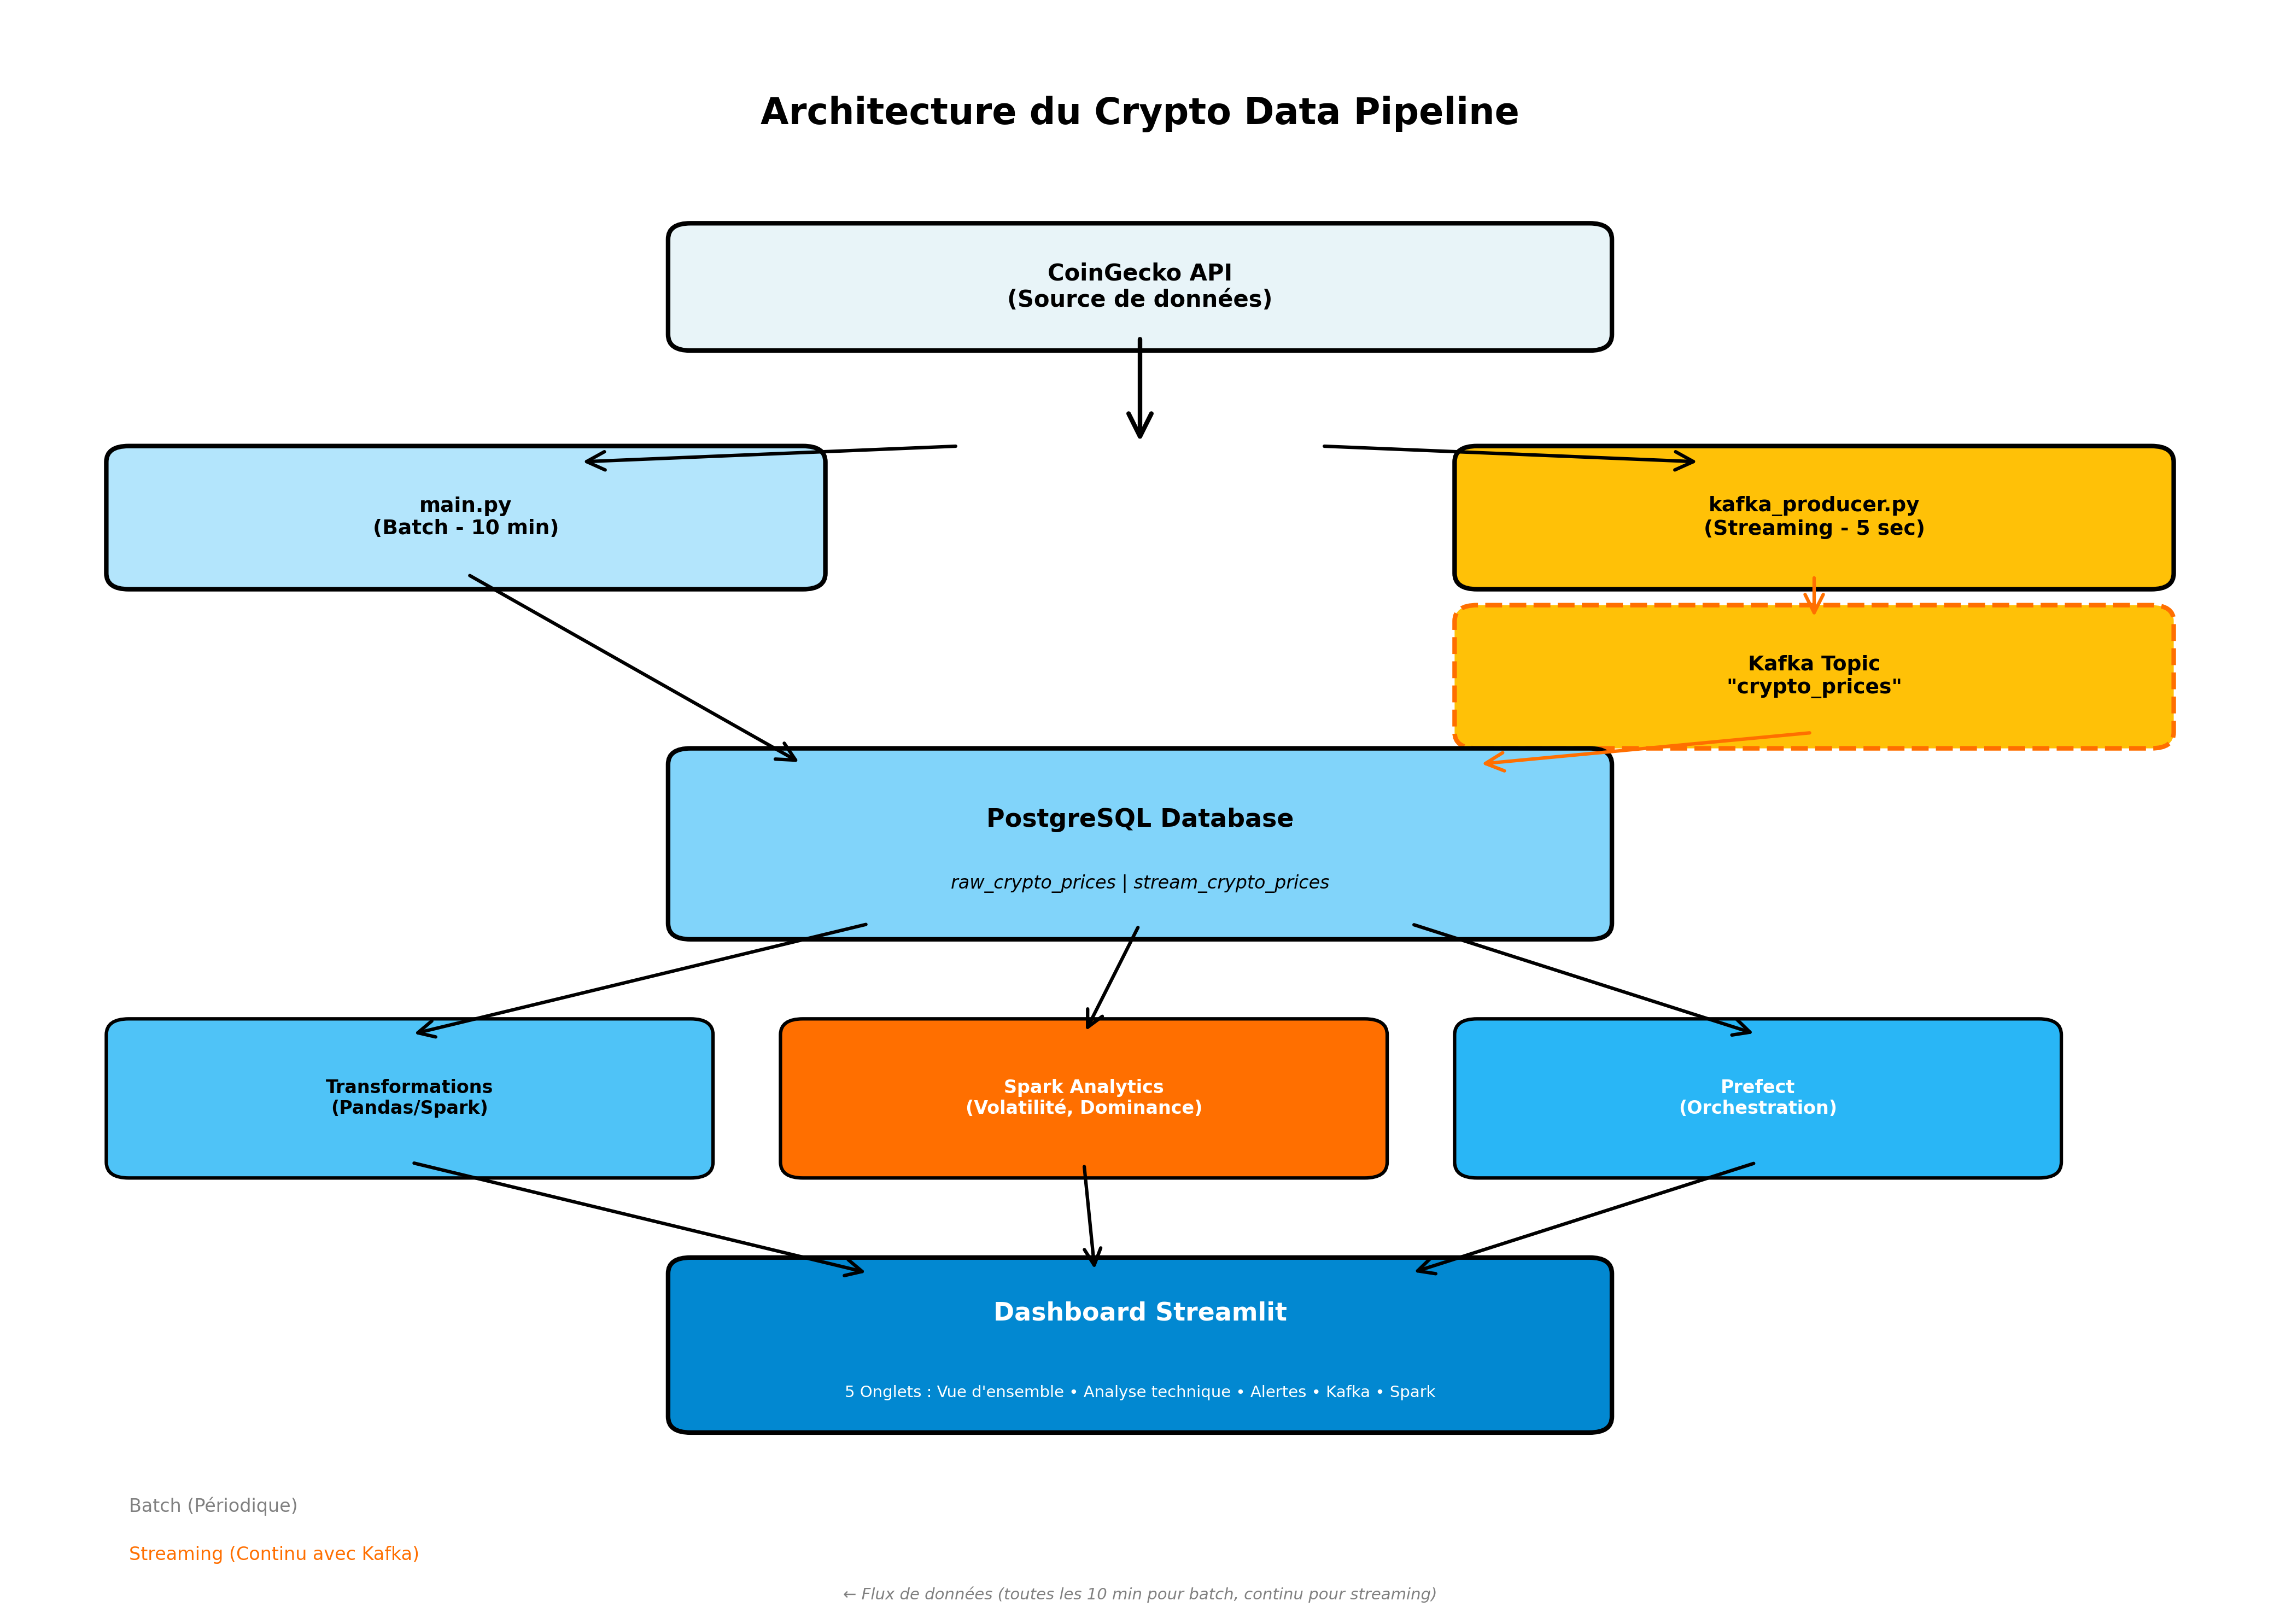
\includegraphics[width=0.95\textwidth]{figures/architecture_diagram.png}
    \caption{Architecture globale du pipeline}
    \label{fig:architecture}
\end{figure}

\textbf{Couche d'ingestion :} Batch (main.py, API CoinGecko) + Streaming (Kafka producer/consumer)

\textbf{Couche de stockage :} PostgreSQL 15 (Docker local) / Neon Cloud (production). Tables : \texttt{raw\_crypto\_prices}, \texttt{stream\_crypto\_prices}, \texttt{transform\_*}.

\textbf{Couche de transformation :}
\begin{itemize}[noitemsep]
    \item \textbf{Pandas} : nettoyage, agrégations, alertes (pour < 50k lignes)
    \item \textbf{PySpark} : transformations scalables + Spark SQL (volatilité, dominance marché)
\end{itemize}

\textbf{Couche d'orchestration :} Prefect (planification, retry automatique)

\textbf{Couche de visualisation :} Streamlit v1.42 + Plotly (5 onglets interactifs, dark theme)

\subsection{Flux de Données Détaillé}

\begin{figure}[H]
    \centering
    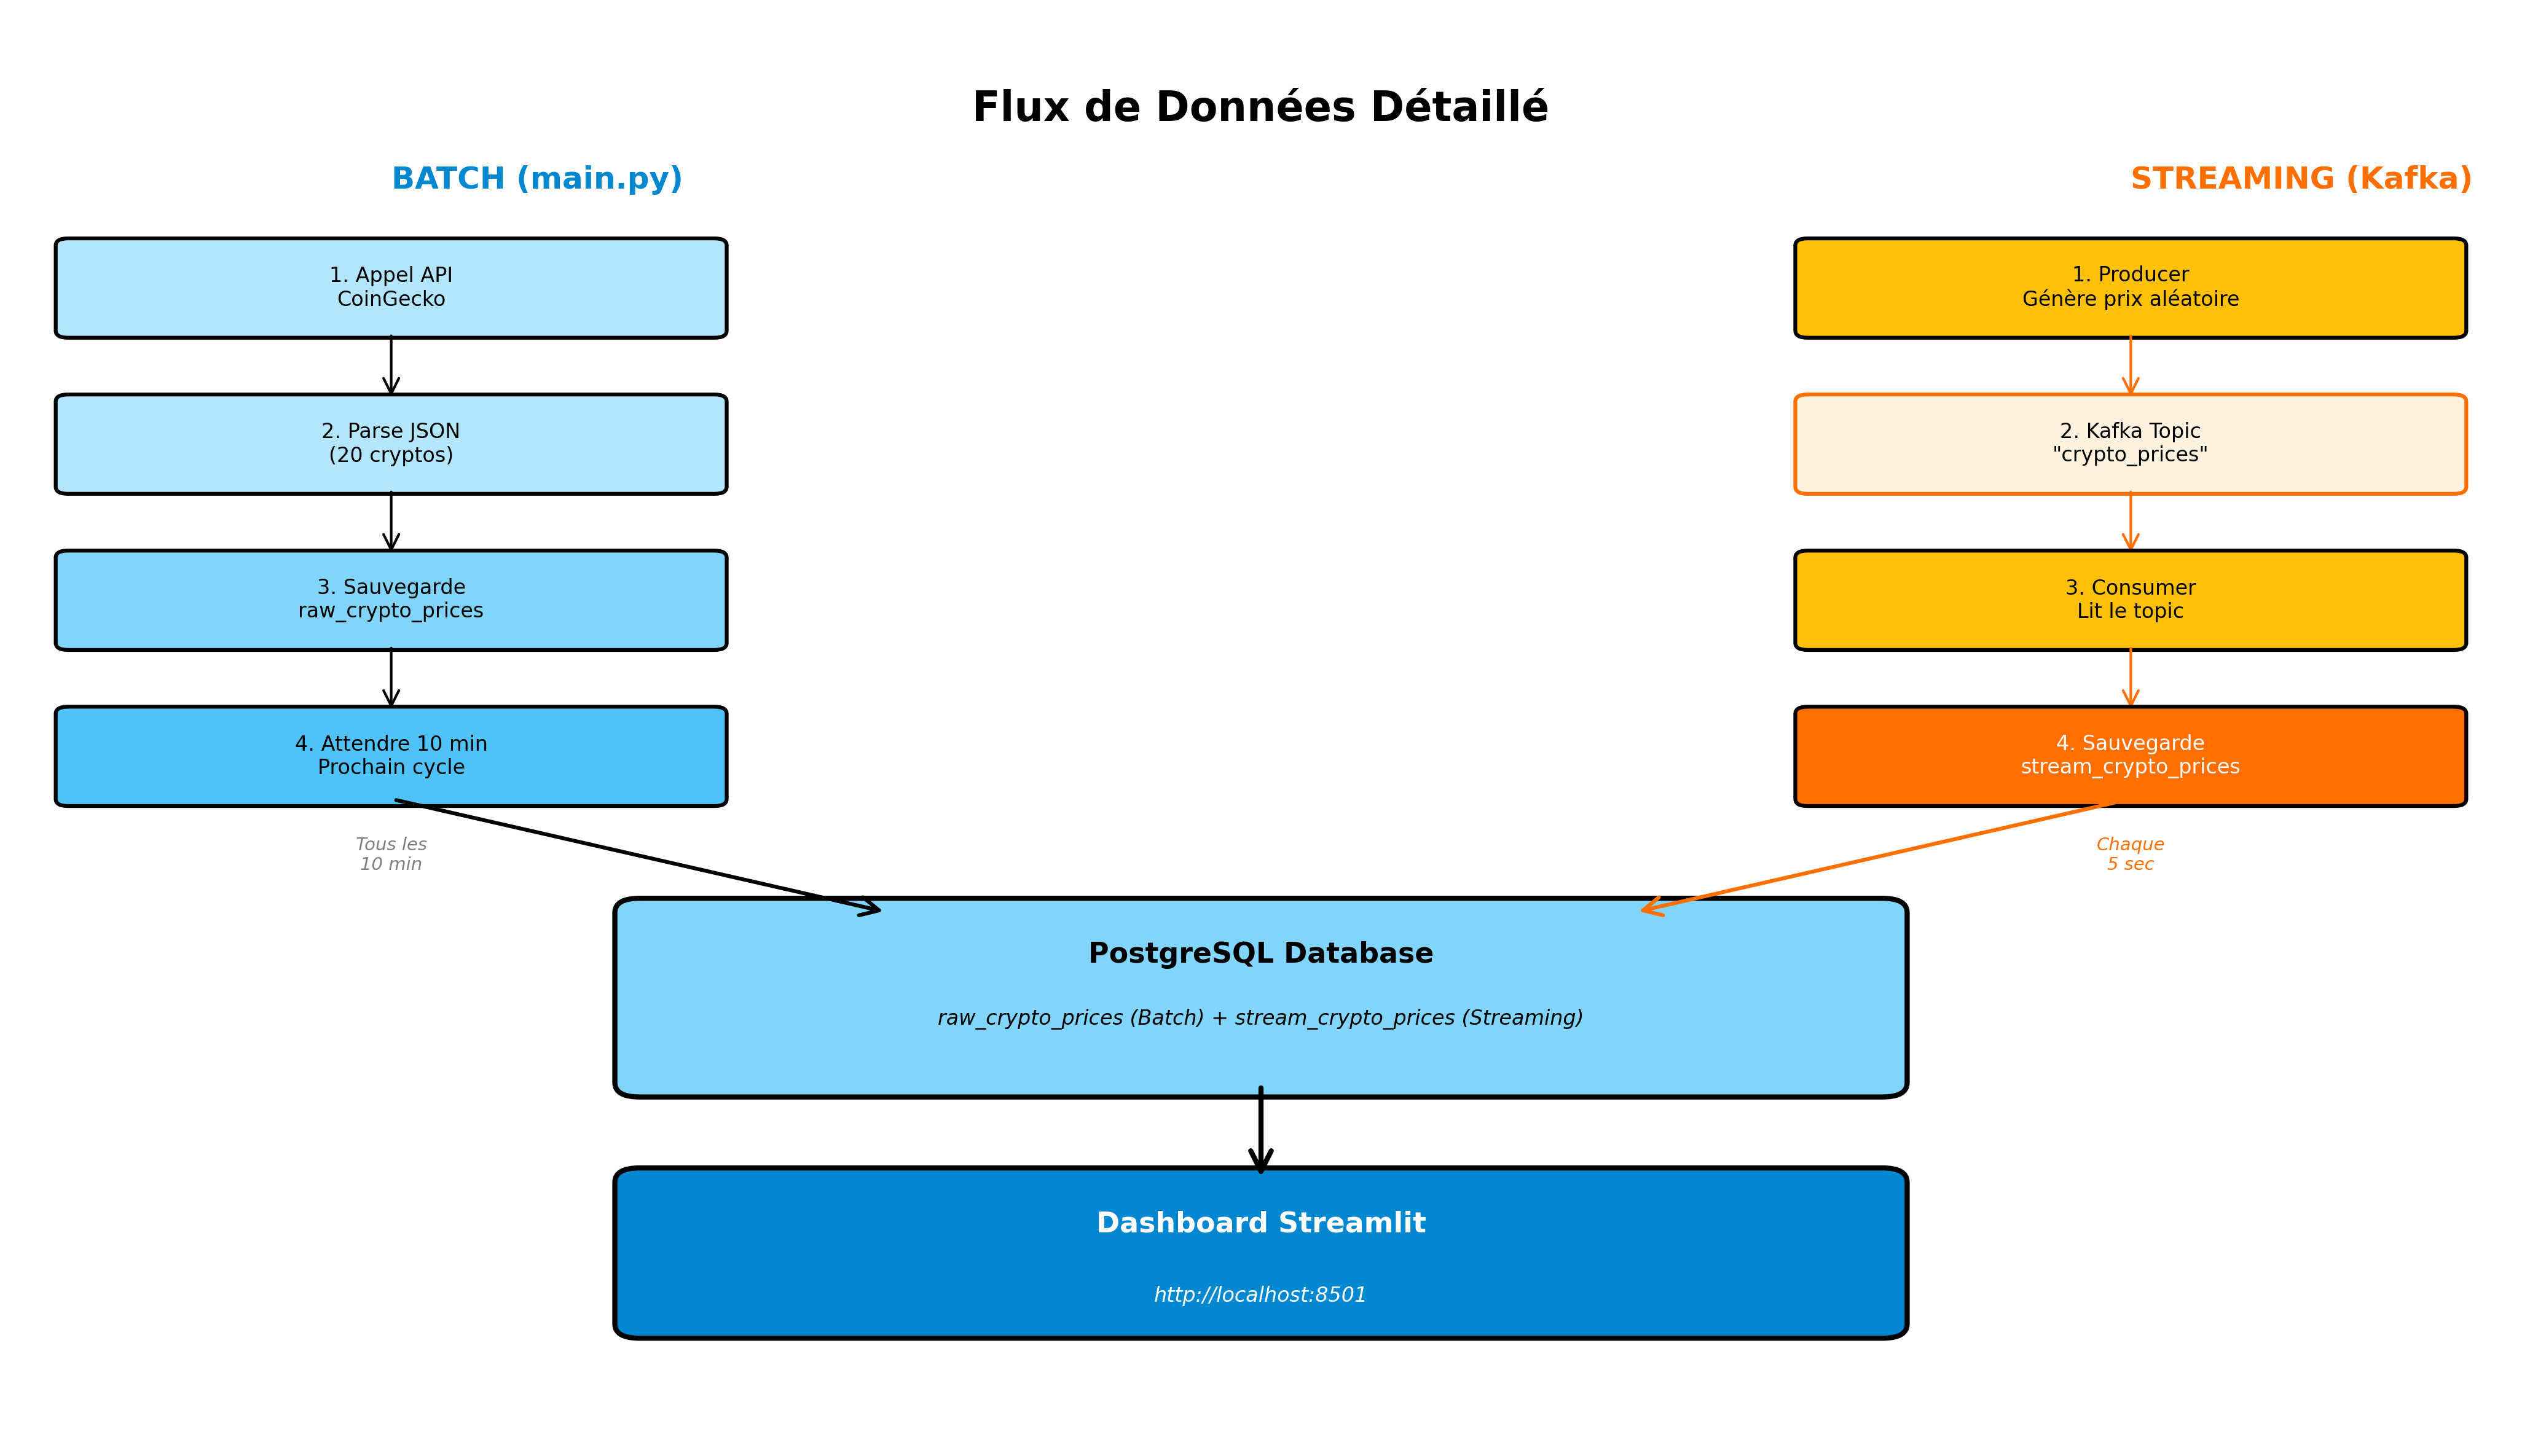
\includegraphics[width=0.95\textwidth]{figures/data_flow_diagram.png}
    \caption{Flux de données : chemins batch et streaming}
    \label{fig:dataflow}
\end{figure}

Deux chemins parallèles : \textbf{Batch} (10 min, complet) alimente \texttt{raw\_crypto\_prices}, \textbf{Streaming} (5 sec, continu) alimente \texttt{stream\_crypto\_prices}. Les deux convergent vers PostgreSQL puis le dashboard.

% ===== 4. STACK ET ARCHITECTURE DUAL-ENGINE =====
\section{Stack Technologique et Architecture Dual-Engine}

\begin{table}[H]
\centering
\small
\begin{tabular}{|l|p{6.5cm}|}
\hline
\textbf{Couche} & \textbf{Technologie} \\
\hline
Ingestion & Python + CoinGecko API + Kafka \\
\hline
Stockage & PostgreSQL 15 / Neon Cloud \\
\hline
Transformation (Pandas) & Pandas 2.2.3 (< 50k lignes) \\
\hline
\textbf{Transformation (Spark)} & \textbf{PySpark 3.5.1 ($\geq$ 50k lignes)} \\
\hline
Orchestration & Prefect 3.x \\
\hline
Visualisation & Streamlit 1.42 + Plotly 5.24 \\
\hline
Déploiement Dev & Docker Compose \\
\hline
\end{tabular}
\caption{Stack technologique}
\end{table}

\subsection{Architecture Dual-Engine}

Le projet implémente une sélection \textbf{automatique} du moteur de traitement selon le volume :

\begin{lstlisting}[language=Python]
def auto_select_engine(nb_rows: int, threshold: int = 50_000) -> str:
    return "spark" if nb_rows >= threshold else "pandas"
\end{lstlisting}

\textbf{Avantages :} Pas de surcharge Spark sur petits volumes, scalabilité garantie si volume $\geq$ 50k. Les Window Functions Spark (classement, partitionnement) outpassent Pandas pour les analytics avancées.

% ===== 5. TRANSFORMATIONS MÉTIER =====
\section{Transformations Métier}

Cinq transformations implémentées en Pandas ET PySpark :

\begin{itemize}[noitemsep]
    \item \textbf{Nettoyage :} Suppression NULL, doublons, valeurs aberrantes
    \item \textbf{Agrégations :} Moyenne/min/max horaires et journaliers (GROUP BY)
    \item \textbf{Classements :} Ranking par variation 24h (Window Functions Spark)
    \item \textbf{Alertes :} Détection HAUSSE ($\geq +5\%$), BAISSE ($\leq -5\%$)
    \item \textbf{Analyses avancées} : Volatilité (STDDEV), dominance marché (Spark SQL)
\end{itemize}

% ===== 6. INTÉGRATION APACHE SPARK =====
\section{Intégration Apache Spark}

\subsection{Gestion de la SparkSession}

Trois nouveaux fichiers : \texttt{spark\_engine.py} (gestion SparkSession singleton), \texttt{spark\_transformations.py} (implémentations PySpark), \texttt{run\_transforms.py} (sélection auto moteur).

\begin{lstlisting}[language=Python]
# spark_engine.py
SparkSession.builder.appName("CryptoDataPipeline")
    .master("local[1]")
    .config("spark.driver.memory", "1g")
    .config("spark.sql.execution.arrow.pyspark.enabled", "false")
    .getOrCreate()
\end{lstlisting}

Configuration Windows : \texttt{local[1]} (1 thread) + Arrow désactivé (évite crash Python 3.12).

\subsection{Analyses Spark SQL}

\textbf{Volatilité :} Écart-type des prix par crypto -- démontre Spark SQL avancé.

\textbf{Dominance de marché :} Pourcentage du market cap total (Window Functions : \texttt{ROW\_NUMBER()}, \texttt{SUM() OVER()}).

\textbf{Solution Windows :} Conversion Pandas→Spark via fichier CSV temporaire (évite crash sérialisation Python 3.12 avec Py4J).

% ===== 7. DASHBOARD STREAMLIT =====
\section{Dashboard Streamlit -- Version 2.1}

\subsection{Interface 5 Onglets}

\begin{table}[H]
\centering
\small
\begin{tabular}{|l|p{6cm}|}
\hline
\textbf{Onglet} & \textbf{Contenu} \\
\hline
📊 Vue d'ensemble & KPI cards, évolution des prix, classement journalier \\
\hline
📈 Analyse technique & Chandelier OHLC, heatmap corrélation, performance relative \\
\hline
⚠️ Alertes \& Volume & Alertes volatilité, variations 24h, volume time-series \\
\hline
⚡ Streaming Kafka & Prix temps réel, distribution variations, événements \\
\hline
🔥 Spark Analytics & Volatilité (Spark SQL), dominance (SQL), tableaux \\
\hline
\end{tabular}
\caption{Onglets du dashboard}
\end{table}

\textbf{Améliorations v2.1 :} Dark theme professionnel (\texttt{\#0f1117}), KPI cards stylisées, graphique candlestick OHLC (calcul Open/High/Low/Close horaires), heatmap corrélation, Spark Analytics tab (analyses via SQL PostgreSQL, sans Spark local sur cloud).

URL : \url{https://crypto-data-pipeline-8mrtpexxnwydrp9dbehvt5.streamlit.app}

% ===== 8. DÉPLOIEMENT =====
\section{Déploiement}

\textbf{Développement :} PostgreSQL + Kafka + Spark en Docker Compose local.

\textbf{Production :}
\begin{itemize}[noitemsep]
    \item Base de données : Neon PostgreSQL Cloud (gratuit)
    \item Dashboard : Streamlit Cloud (gratuit, auto-refresh 60s)
    \item Analyses Spark : calculées via SQL PostgreSQL (pas Spark sur cloud = économie ressources)
\end{itemize}

\textbf{Reproductibilité :} \texttt{docker-compose.yml} + \texttt{requirements.txt} (PySpark exclu de Cloud, non nécessaire).

% ===== 9. TESTS ET DIFFICULTÉS =====
\section{Tests et Difficultés Résolues}

\subsection{Tests}
18 tests unitaires couvrent les transformations Pandas (nettoyage, agrégations, alertes, classement). \textbf{Résultat :} 18/18 passés ✓

\subsection{Principales Difficultés}

\textbf{1. PySpark Crash Windows (Python 3.12) :} \texttt{createDataFrame(pandas\_df)} provoque \texttt{EOFException} (incompatibilité Py4J). \textbf{Solution :} Conversion via CSV temporaire (Pandas→CSV→Spark JVM).

\textbf{2. CoinGecko 403 Forbidden :} API nécessite clé depuis 2024. \textbf{Solution :} Inscription gratuite + header \texttt{x-cg-demo-api-key}.

\textbf{3. Déploiement cloud :} Streamlit Cloud ne peut accéder PostgreSQL local. \textbf{Solution :} Migration Neon + script \texttt{migrate\_to\_neon.py}.

\textbf{4. background\_gradient matplotlib absent :} Streamlit Cloud n'a pas matplotlib. \textbf{Solution :} \texttt{.map()} avec CSS conditionnelle.

% ===== 10. RÉSULTATS =====
\section{Résultats et Fonctionnalités}

\textbf{Métriques :}
\begin{itemize}[noitemsep]
    \item Données collectées : $\sim$5 050 lignes (7 jours)
    \item Fréquence : 10 min (batch) + 5 sec (streaming)
    \item Uptime : 24/7 via Streamlit Cloud
    \item Latence requête BD : < 2 sec
    \item Tests : 100\% (18/18)
\end{itemize}

\textbf{Fonctionnalités délivrées :}
\begin{itemize}[noitemsep]
    \item Pipeline automatisé end-to-end ✓
    \item Dashboard accessible publiquement ✓
    \item Alertes automatiques ✓
    \item \textbf{Architecture dual-engine Pandas/Spark [Nouveau]} ✓
    \item \textbf{Analyses Spark SQL : volatilité, dominance [Nouveau]} ✓
    \item \textbf{Dashboard dark theme 5 onglets [Nouveau]} ✓
\end{itemize}

% ===== 11. CONCLUSION =====
\section{Conclusion}

Ce projet démontre la maîtrise d'une \textbf{chaîne Data Engineering complète et production-ready} : ingestion (batch + streaming Kafka), stockage cloud (Neon PostgreSQL), transformation dual-engine (Pandas/Spark avec sélection automatique), orchestration (Prefect), et visualisation professionnelle (Streamlit 5 onglets).

L'intégration d'\textbf{Apache Spark} constitue l'élément technique avancé : architecture dual-engine intelligente, Window Functions pour classements scalables, Spark SQL pour analyses volatilité/dominance. La gestion du crash Python 3.12/PySpark 3.5 via CSV temporaire démontre capacité de troubleshooting en production.

Le \textbf{dashboard v2.1} offre expérience utilisateur de niveau professionnel avec dark theme, 5 onglets thématiques, graphiques interactifs (Plotly), et intégration Spark Analytics.

\textbf{Compétences acquises :} Ingestion batch+streaming, stockage relationnel cloud, transformations Pandas ET PySpark, Spark SQL, orchestration Prefect, déploiement cloud, dashboard interactif, tests unitaires.

\textbf{Pipeline opérationnel 24/7 :} \url{https://crypto-data-pipeline-8mrtpexxnwydrp9dbehvt5.streamlit.app}

\newpage
\section*{Annexes}

\subsection*{Annexe A -- Structure du Projet}
\texttt{ingestion/} (main.py, kafka, database.py), \texttt{transformations/} (cleaning, spark\_engine.py, spark\_transformations.py), \texttt{dashboard/} (app.py), \texttt{orchestration/} (Prefect flows), \texttt{tests/}, \texttt{docker-compose.yml}, \texttt{requirements.txt}

\subsection*{Annexe B -- Dépôt et Resources}
GitHub : \url{https://github.com/asmasebai123/crypto-data-pipeline}\\
Dashboard : \url{https://crypto-data-pipeline-8mrtpexxnwydrp9dbehvt5.streamlit.app}

\end{document}
